\documentclass[]{article}
\usepackage[russian, spanish.mexico]{babel}
\usepackage[T1]{fontenc}
\usepackage[utf8]{inputenc}
%\usepackage{lmodern}
\usepackage[a4paper]{geometry}
 \geometry{
	a4paper,
	%total={170mm,257mm},
	left=15mm,
	right=15mm,
	%top=20mm,
}

%DIAGRAMAS
\usepackage{smartdiagram}
\usesmartdiagramlibrary{additions}
%ARBOLES
%\usetikzlibrary{trees}

%Plotting

\usepackage{pgfplots}
\pgfplotsset{width=10cm,compat=1.9} 
%\usepgfplotslibrary{external}
%\tikzexternalize 

%Graficos e imagenes
\usepackage{graphicx}
%\graphicspath{ Imagenes/ }
\usetikzlibrary{arrows}

\usepackage{natbib}
\usepackage{cite}

\usepackage{subcaption}

%columnas itemize
\usepackage{multicol}

%Grafico de barras
%\usepackage{pgfplots}
%Arrreglos
\usepackage{array}

\usepackage{tikz}
\usepackage[american voltages, american currents,siunitx]{circuitikz}

\title{Reactores VVER}
\author{Pablo Vivar Colina}
%Comentar para obtener fecha de HOYs
%\date{Octubre 2019}


\begin{document}
	
%%\usepackage[top=2cm,bottom=2cm,left=1cm,right=1cm]{geometry}


\begin{titlepage}
     \begin{center}
	
\includegraphics[width=0.09\textwidth]{UNAM}\Large Universidad Nacional Autónoma de México
        	
\includegraphics[width=0.09\textwidth]{FI}\\[1cm]
        \Large Facultad de Ingeniería\\[1cm]
       % \Large División de Ciencias Básicas\\[1cm]
         \Large Laboratorio de Fundamentos de Control(6655)\\[1cm]
         %la clave antes era:4314
         \footnotesize Profesor: Salcedo Ubilla María Leonor Ing.\\[1cm]
        \footnotesize Semestre 2019-1\\[1cm]
        
       

        \Large Práctica No. 1\\[1cm]
        
           

\Large Introdcción MATLAB
        
         %Texto a la derecha
          \begin{flushright}
\footnotesize  Grupo 2\\[0.5cm]
\footnotesize Brigada: 4\\[0.5cm]
\footnotesize Rodrigo Adrián Martínez López\\[0.5cm]
\footnotesize Vivar Colina Pablo\\[0.5cm]
 \end{flushright}
    %Texto a la izquierda
          \begin{flushleft}
        \footnotesize Ciudad Universitaria Agosto de 2018.\\
          \end{flushleft}
         
          
        %\vfill
        %\today
   \end{center}
\end{titlepage}
 %agregar portada

\maketitle

\tableofcontents  % Write out the Table of Contents

\listoffigures  % Write out the List of Figures

%#Puntos cubiertos en el proyecto

\section{Introducción}


El reactor agua-agua-energía (WWER),o VVER (del ruso: 

\selectlanguage{russian}

вод-водяной энергетический реактор

\selectlanguage{spanish}

transliterado como vodo-vodyanoi energetichesky reaktor; reactor agua-agua-energía) es una serie de diseños de reactores de agua a presión desarrollados originalmente en la Unión Soviética, y ahora en Rusia, por OKB Gidropress La idea de un reactor fue propuesta en el Instituto Kurchatov por Savely Moiseevich Feinberg. Los VVER se desarrollaron originalmente antes de la década de 1970 y se han actualizado continuamente. Como resultado, el nombre VVER se asocia con una amplia variedad de diseños de reactores que abarcan desde reactores de la generación I hasta diseños modernos de la generación III+. La potencia va de 70 a 1300 MWe, con diseños de hasta 1700 MWe en desarrollo[3][4] El primer prototipo VVER-210 se construyó en la central nuclear de Novovoronezh.\\

Las centrales VVER se han instalado principalmente en Rusia y la antigua Unión Soviética, pero también en China, Finlandia, Alemania, Hungría, Eslovaquia, Bulgaria, India e Irán. Los países que están planeando introducir reactores VVER son Bangladesh, Egipto, Jordania y Turquía.\citep{BaezaG.2009}\\

Los reactores VVER de ROSATOM se encuentran entre los reactores más utilizados del mundo. Las plantas VVER han demostrado su alta fiabilidad en más de 1300 reactores-año de funcionamiento. Desde la puesta en servicio de la primera unidad de potencia VVER en los años 60, la tecnología ha estado proporcionando electricidad segura y asequible en todo el mundo: desde las montañas armenias hasta el campo de la República Checa, por encima del Círculo Polar Ártico y en el extremo sur de la India.\citep{Rosatom}\\

\subsection{Diseños de reactores rusos}

Mientras que los Estados Unidos y Europa Occidental
persiguieron LWRs de diseños algo similares, la antigua Unión Soviética y los antiguos países del Bloque del Este desarrollaron sus propios diseños únicos. Estos diseños incluyen los reactores RBMK y VVER. Ambos han encontrado una amplia aplicación en la antigua Unión Soviética, en los antiguos países del Bloque Oriental y en otros lugares. Tienen varias características únicas que no se encuentran en los diseños de reactores occidentales.\citep{Lamarsh2001}

\subsubsection{Reactores VVER}

Se pusieron en operacion en 1970, la serie de reactores VVER 440 generaban 440MWe, Todos estos reactores de diseño tienen seis lazos, una válvula de aislamiento en cada lazo y un tubo horizontal de gereación de vapor con un diseño único. El NSSS maneja turbinas de vapor de 220MEe. Condiciones de operación del VVER se muestran en el cuadro \ref{parametrosVVER}.\\

El diseño del núcleo del reactor difiere de la mayoría de los diseños occidentales, ya que usa ensamblajes hexgonales para el combustible. Cada ensamblaje de combustible enstá envuelto por una cubierta similar a los BWR estadounidenses. El núcleo consiste en 312 ensamblajes de combustible y 37 ensamblajes de control móviles. Los ensamblajes de control tienen seguidores de combustible que entran en la sección superior del núcleo que contiene también el material de control compuesto por acero de boro.Cada ensamble consiste en 126 barras de combustible, cada una acomodada en froma triangular, la barra de combustible tiene 9.1mm de diámetro y contiene 7.5mm de diámetro de UO2, las pastillas de combustible enriquecidas de 2.4 a 2.6 3/o. Las barras de combustibles son de 3.53 m de largo. Adicionalmente el control se hace a través de ácido bórico así como en los PWR occidentales.\citep{Lamarsh2001}\\
 

 %TABLA LLENADA CON VALORES DE WIIKIPEDIA
\begin{table}[h!]
	\centering
	\begin{tabular}{|c|c|c|}
		\hline
		
		         & VVER-440 & VVER-1000 \\ \hline
		Potencia & 1375 MWt & 3000 MWt \\ \hline
		Altura del núcleo & 2.5 m & 3.5 m \\ \hline
		Diametro del núcleo & 2.88 m & 3.12 \\ \hline
		Enriquecimiento de combustible & 3.5$\%$ & 4.26 $\%$\\ \hline
		%Temperatura del refrigerante & $^oC$ &\\ \hline
		tubo de entrada & 269 $^oC$ & 289 $^oC$  \\ \hline
		tubo de salida & 300 $^oC$ & 319 $^oC$ \\ \hline
		Presión de vapor & 125 $\frac{Kg}{cm^2}$ & 160 $\frac{Kg}{cm^2}$ \\ \hline
		Presión de sistema de refrigeración &  44 $\frac{Kg}{cm^2}$ & 60 $\frac{Kg}{cm^2}$\\ \hline
	\end{tabular}
  \caption{Parámetros VVER}
  \label{parametrosVVER}
\end{table}

%para minimizar la presión de contención durante los LOCA. La figura 4.2 1 muestra la disposición del sistema de refrigeración y contención del reactor para un VVER 213.\\

El reactor más grande de la serie VVER 1 OOO es un PWR de cuatro lazos que se asemeja mucho al un PWR occidental estándar. Con una potencia nominal de 1.000 MWe, estos reactores entraron en servicio a mediados de la década de 1980. Se diferencian de la serie de diseño 440 en que utilizan una conexión similar a los PWR occidentales y tienen cuatro lazos con un generador de vapor en cada lazo. Al igual que los reactores VVER 440, los VVER 1000s utilizan generadores de vapor horizontales y dos turbinas.\\

\begin{figure}[h!]
	\centering
	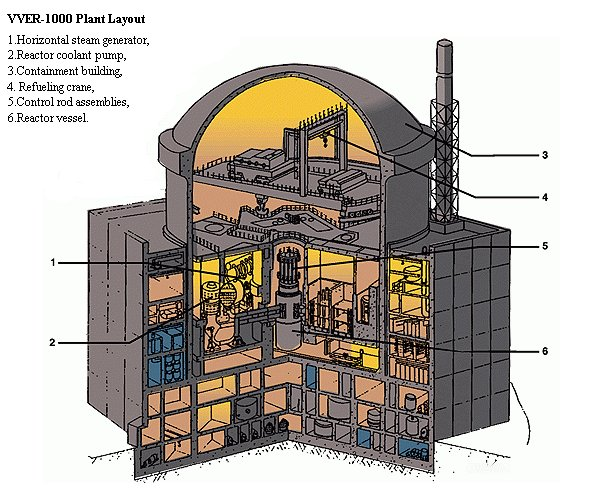
\includegraphics[width=0.8\textwidth]{vver-1000-layout}
	\caption{VVER 1000}
	\label{fig:VVER_1000}
\end{figure}

La figura \ref{fig:VVER_1000} muestra la disposición de un VVER 1000 típico. Al igual que el VVER 440, el VVER 1000 utiliza elementos de combustible hexagonales. El
Sin embargo, los elementos de combustible de la serie 1000 son mucho más grandes que los del diseño VVER 440 y no tienen cubiertas de elementos de combustible. El combustible también utiliza una zonificación del enriquecimiento con pines de combustible de menor enriquecimiento ubicados en la periferia de
\citep{Lamarsh2001}\\

\section{Reactores VVER-1200}

En la figura \ref{fig:DiagramaVVER} podemos apreciar el diagrama esquemático de un reactor VVER más moderno a comparación del VVER, en é podemos apreciar los signos de referencia que a continuación serán enlistados.\\

\begin{figure}[h!]
	\centering
	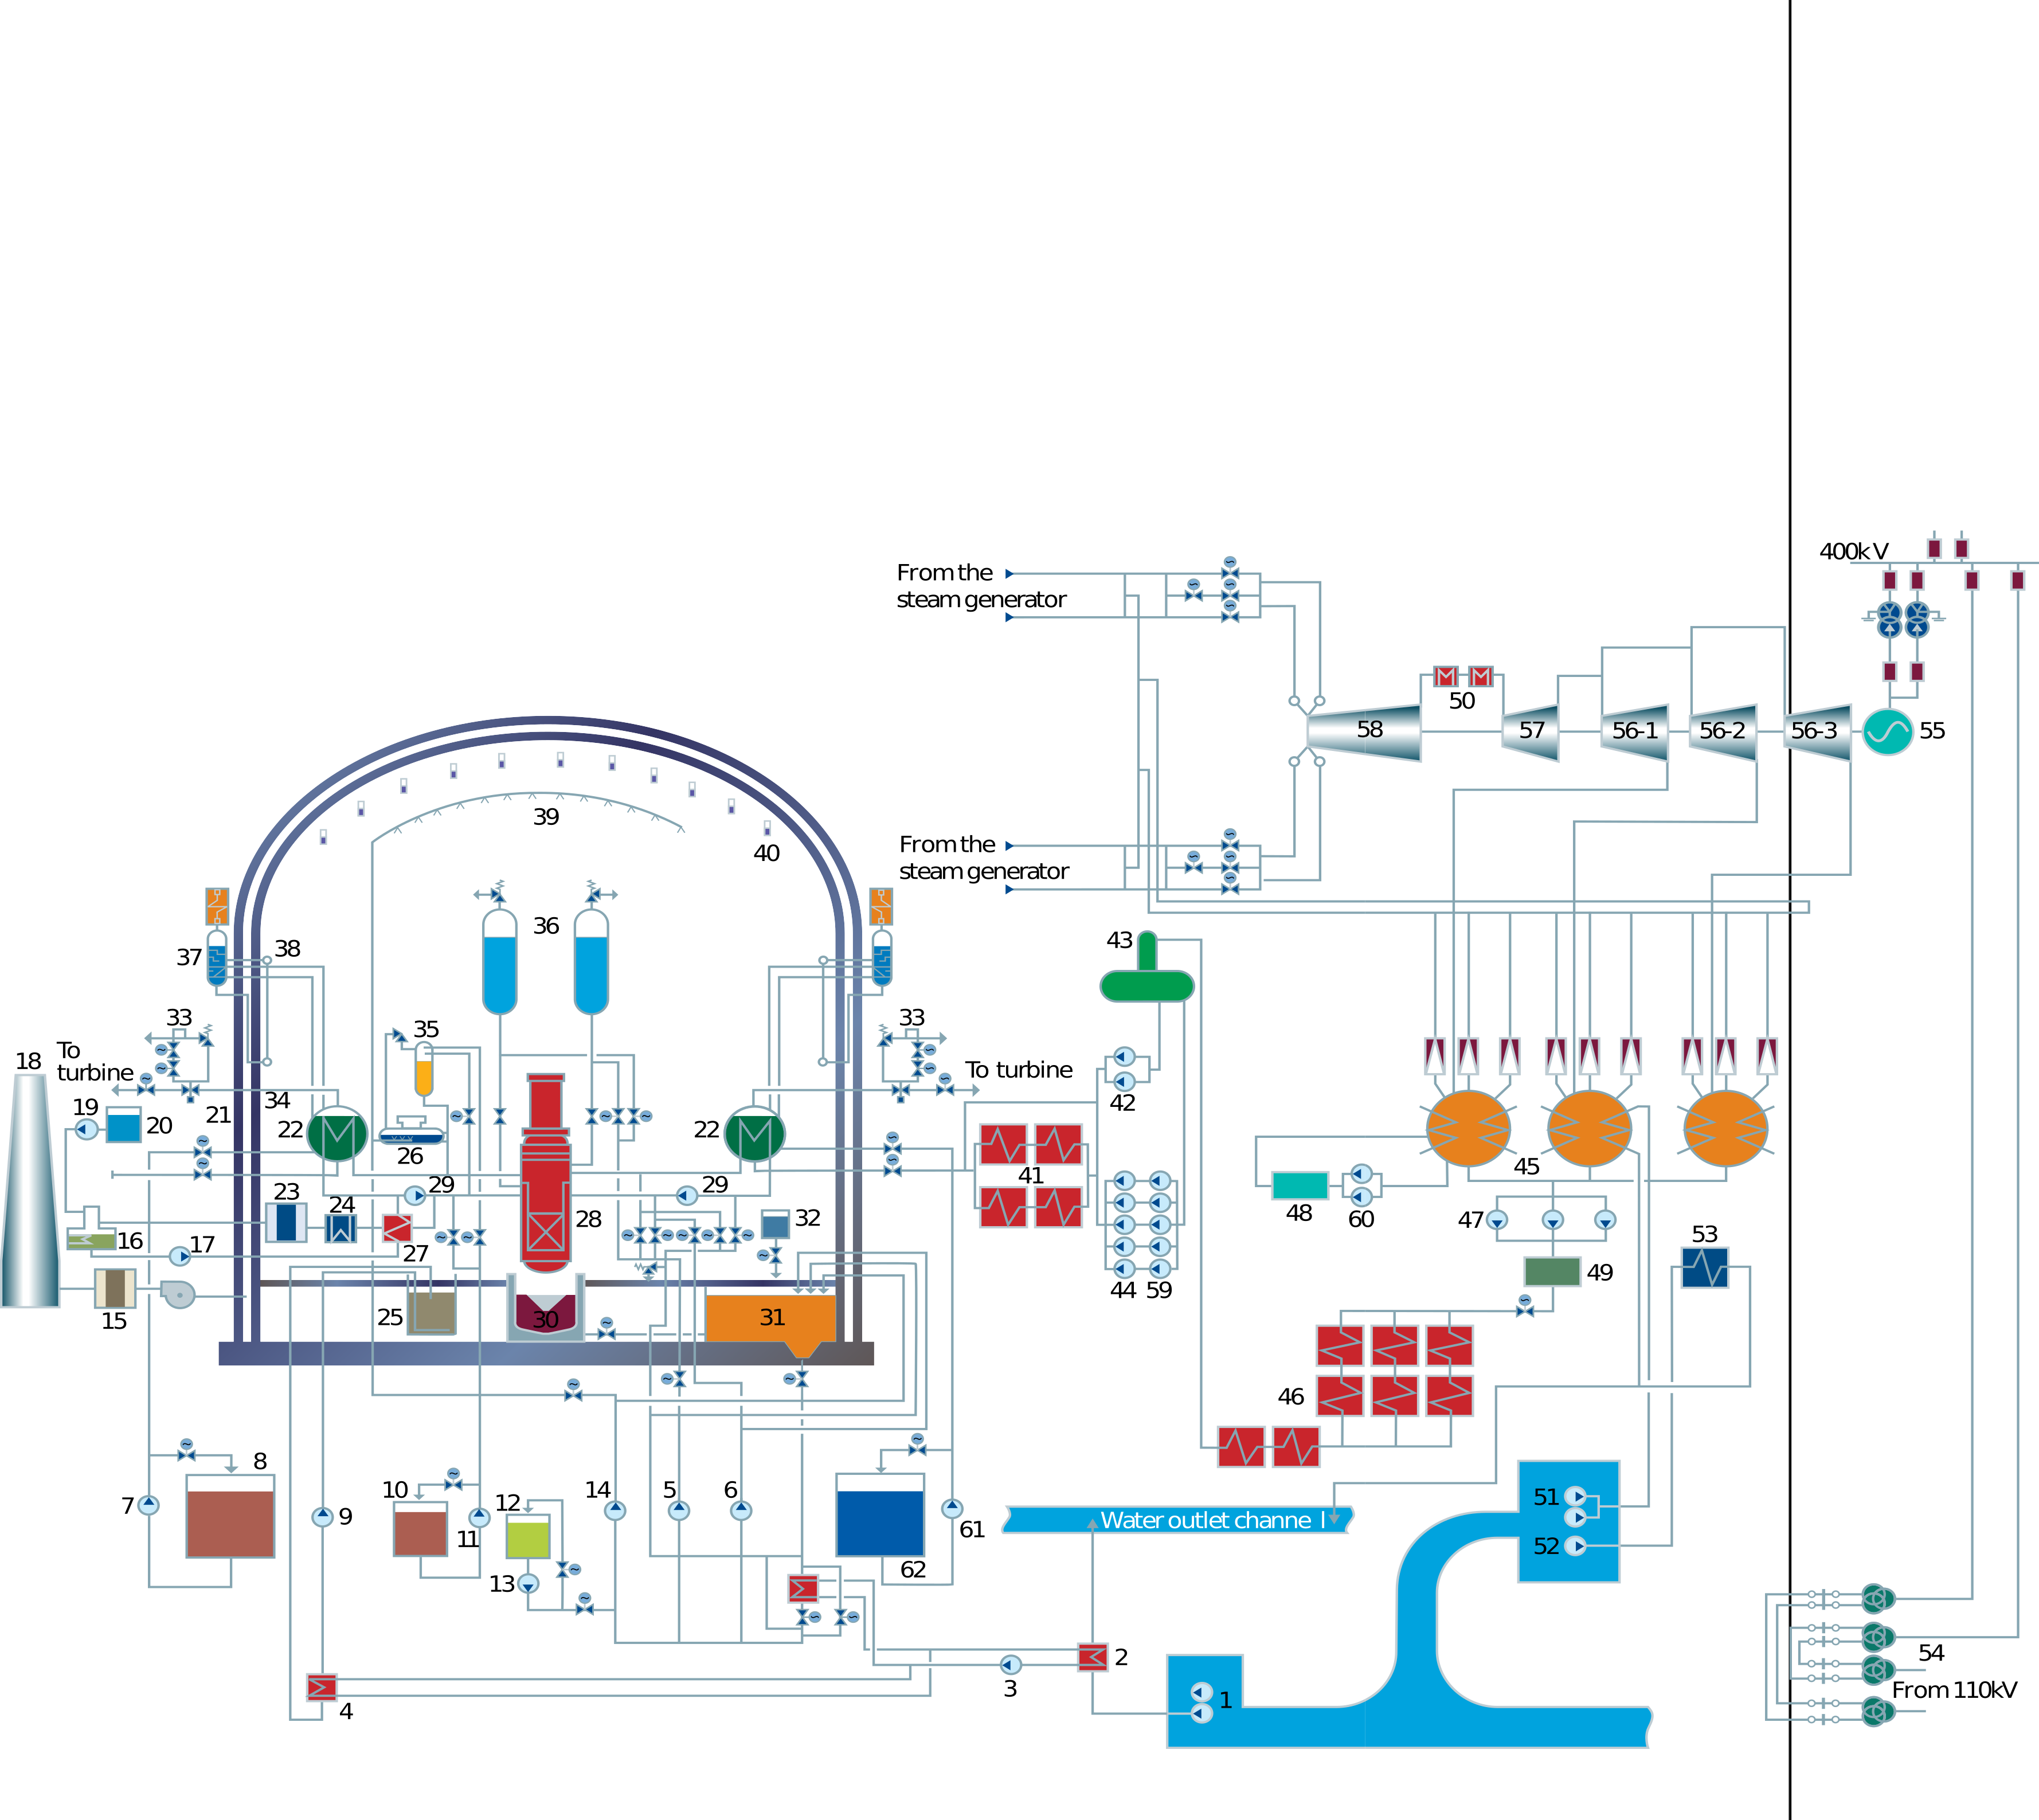
\includegraphics[width=0.95\textwidth]{DiagramaReactorVVER}
	\caption{Diagrma Esquemático Simplificado \citep{Rosatom}}
	\label{fig:DiagramaVVER}
\end{figure}


\begin{multicols}{2}
	\begin{enumerate}
		\item Bomba de agua de refrigeración esencial (o "agua de servicio")
		\item Intercambiadores de calor del circuito intermedio de refrigeración para consumidores prioritarios
		\item Bomba del circuito intermedio
		\item Intercambiador de calor de la piscina de combustible gastado
		\item Sistema de inyección de emergencia, bomba de baja presión
		\item Sistema de inyección de emergencia, bomba de alta presión
		\item Bomba de agua de alimentación de emergencia
		\item Tanques de almacenamiento para ácido bórico de alta concentración
		\item Bomba de refrigeración de combustible gastado
		\item Tanques de almacenamiento para solución de ácido bórico
		\item Bomba del sistema de boración de emergencia
		\item Tanque de almacenamiento de reactivos químicos
		\item Bomba de suministro para reactivos químicos
		\item Bomba del sistema de rociado de contención
		\item Filtrante
		\item Purgador de aire del sistema de control de volumen y químico
		\item Bomba del sistema de control de volumen y de productos químicos
		\item Chimenea de ventilación
		\item Bomba con fugas controladas
		\item Depósito con fugas controladas
		\item Contención externa
		\item Generador de vapor
		\item Planta de tratamiento
		\item Refrigerador posterior
		\item Piscina de combustible gastado
		\item Tanque de ebullición
		\item Intercambiador de calor regenerativo para el sistema de control de volumen y químico
		\item Reactor
		\item Bomba de refrigerante del reactor
		\item Captador de núcleos
		\item Sistema de enfriamiento de emergencia del núcleo del sumidero y tanque de almacenamiento de agua de reabastecimiento de combustible
		\item Tanque de reserva de emergencia de álcali (NaOH)
		\item MSIV, conjunto de válvulas de seguridad y alivio
		\item Confinamiento
		\item Presurizador
		\item Hidroacumuladores ECCS
		\item Tanque del sistema de remoción de calor pasivo
		\item Condensador para el sistema de eliminación pasiva de calor de contención
		\item sistema de rociado
		\item Recombinador pasivo de hidrógeno
		\item Calentadores de alta presión
		\item Bomba de agua de alimentación auxiliar eléctrica
		\item Purgador de aire
		\item Bomba de agua de alimentación eléctrica
		\item Condensador
		\item Calentadores de baja presión
		\item Bombas de condensado, primera etapa
		\item Unidad de planta de agua desmineralizada
		\item Tratamiento principal de condensados
		\item Sobrecalentador
		\item Bombas de agua de refrigeración de circulación
		\item Bomba de agua de refrigeración para los consumidores de la sala de turbinas
		\item Consumidores de sala de turbinas
		\item Transformador reductor de tensión de reserva
		\item Grupo electrógeno
		\item Cilindros de baja presión de turbina
		\item Cilindro de presión intermedia de la turbina
		\item Cilindro de alta presión de la turbina
		\item Bomba de impulsión
		\item Bombas de condensado para plantas de desmineralización de unidades
		\item Bomba de agua de alimentación de emergencia
		\item Tanque de almacenamiento de agua desmineralizada
	\end{enumerate}
\end{multicols}

%\section{Combustible}
%Tipo de combustible y formatos(enriquecimiento, pastillas, geometría)

%\section{Moderador}
%Moderador (si existe o no) para un reactor rápido no necesita

\subsection{Refirgerante}

 \subsubsection{Tubería principal del refrigerante}

La tubería principal del refrigerante (primario) que conecta
el reactor, los generadores de vapor y el refrigerante del reactor
tiene un diámetro nominal, Dnom, de 850 mm,
con una vida útil de 60 años. El valor nominal externo
el diámetro es de 990 mm y el grosor nominal de la pared-
ness es de 70 mm. La longitud total es de 146 m. La principal
está diseñado para satisfacer todas las necesidades
condiciones del concepto de "fuga antes de la rotura": ma-
propiedades teriales, análisis de estrés, inspección en servicio.
y control de fugas.\citep{Rosatom}\\

\subsubsection{Bomba de refrigerante del reactor}

La bomba de refrigerante del reactor (principal), también RCP (Reactor Coolant Pump) es de la GCNA Tipo 1391. La RCP está equipada con un volante de inercia que proporciona un funcionamiento suave de la circulación principal del refrigerante. En escenarios de accidentes con pérdida de potencia. Esto permite un enfriamiento adecuado del reactor hasta que el
el reactor está apagado y el calor de decaimiento ha caído
a un nivel en el que pueda ser eliminado de forma segura y natural.\\

 %El diseño incorpora la experiencia
%de las bombas del tipo GCN-195M empleadas.
%en el reactor V-320 y desde el primer GCNA-1391
%que han funcionado de forma fiable en Tianwan
%desde 2007. 

Los datos básicos de la bomba GCNA-1391 son los siguientes
según se indica: capacidad, 22 000 m 3 /h; altura de elevación, 0,588 MPa;
presión nominal de succión, 16,02 MPa; rpm, 1000;
consumo de potencia, caliente, < 5 MW; potencia con-
Consumo, frío, < 6,8 MW; frecuencia de la corriente de alimentación.
cy, 50 Hz; peso (sin motor), 75,5 t; servicio
vida, 60 años.\\

 El GCNA-1391 es un conjunto de bombas verticales,
que consiste en una bomba centrífuga de una etapa con
un eje mecánicamente sellado y soldado esféricamente.
carcasa forjada y asíncrona de dos velocidades.
motor trifásico con volante de inercia. La refrigeración de la bomba
motor y lubricación de todos los cojinetes
por el agua. Refrigeración y lubricación sin aceite elimi-
nates the risk of oil fire inside the reactor contain-
la construcción de capacidades. El diseño de la junta asegura que los valores nominales de
la fuga a través de la bomba es muy pequeña cuando la
la bomba está parada y no hay refrigeración o agua activa
se inyecta en el sello. Esto elimina la
la bomba como posible causa de la pérdida de refirgernate del reactor.\\

%accidente de la hormiga en caso de pérdida a largo plazo de todos los
%energía eléctrica. Durante el desarrollo de la bomba de-
%se prestó especial atención a la posibilidad de reparación y
%reducción de las necesidades de mantenimiento. La bomba

El diseño permite la sustitución de los componentes principales
sin abrir la junta principal, lo que considera una facilidad en el mantenimiento y la reparación.\citep{Rosatom}\\

\subsection{Ejemplo Balakovo-3}

Agua de refrigeración Balakovo-3 con ácido de boro H3BO3:\\
EFPD = 0: Concentración H3BO3 5,2 $[\frac{g}{Kg}]$ H2O\\
FEPA = 170,1:  Concentración H3BO3 2,7 $[\frac{g}{Kg}]$ H2O\\

La temperatura promedio del combustible por VVER-1000 En potencia Máxima es de 830 C grados.\citep{Nea-1995}\\

\section{Potencia eléctrica y térmica}

\begin{table}[h!]
	\centering
	\begin{tabular}{|c|c|c|c|c|c|c|c|}
		\hline
		Unidad     & Tipo de Reactor & En Red & En Bruto & Construcción & En Red & Comercial & Apagado                            \\ \hline
		Balakovo-1 & VVER-1000/320   & 950 MW & 1000MW   & 1980-12-01   & 1985-12-28    & 1986-05-23    & 2045 previsto                      \\ \hline
		Balakovo-2 & VVER-1000/320   & 950 MW & 1000MW   & 1981-08-01   & 1987-10-08    & 1988-01-12    & 2043                       \\ \hline
		Balakovo-3 & VVER-1000/320   & 950 MW & 1000MW   & 1982-11-01   & 1988-12-25    & 1989-04-08    & 2048                       \\ \hline
		Balakovo-4 & VVER-1000/320   & 950 MW & 1000MW   & 1984-04-01   & 1993-05-12    & 1993-12-22    & 2053                       \\ \hline
		Balakovo-5 & VVER-1000/320   & 950 MW & 1000MW   & 1987-04-01   &               &               &  Sus. 1992 \\ \hline
		Balakovo-6 & VVER-1000/320   & 950 MW & 1000MW   & 1988-05-01   &               &               &  Sus.1992 \\ \hline
	\end{tabular}
\caption{Capacidades reactores VVER Balakovo}
\end{table}
\citep{vverWiki}

\section{Sistemas de seguridad}

Se diseñó la planta VVER-1200 (AES-2006)
para cumplir con los requisitos generales de seguridad rusos
emitidas en 1997, que eran coherentes con la
Grupo Internacional de Seguridad Nuclear del OIEA (INSAG)
recomendaciones. El grupo INSAG recomienda-
de los países en vías de desarrollo.\\

Llamadas centrales nucleares de "Generación (Generación) III",
y la actual norma de seguridad del OIEA en materia nuclear
la seguridad en el diseño de centrales eléctricas, publicada en 2012, construye
con los mismos principios. La seguridad general rusa
también son coherentes con las normas de seguridad
los objetivos especificados por la WENRA (Organización de Europa Occidental)
de Reguladores Nucleares) en 2010 para los nuevos
centrales nucleares.\\

El diseño del VVER-1200 (AES-2006) tiene en cuenta
Condiciones de ampliación del diseño (DEC), de acuerdo con
con la actual norma de seguridad del OIEA. Por lo tanto, todos los nuevos
Las plantas VVER-1200 en construcción ya cuentan con
características de diseño que tienen plenamente en cuenta la
principales "lecciones aprendidas de Fukushima", incluyendo:\\

\begin{itemize}
	\item enfriamiento a largo plazo del núcleo del reactor sin necesidad de electricidad.
	poder calórico;
	\item Eliminación del calor de decaimiento a largo plazo que no depende
	en el disipador primario de calor final (mar, río, refrigeración
	torre;
	\item Protección de la integridad de la contención del reactor con
	sistemas dedicados después de un accidente de fusión del núcleo.
\end{itemize}

Los sistemas de seguridad están diseñados para tener el capacidad para un funcionamiento estable en condiciones adversas
debido a fenómenos naturales como los terremotos,
inundaciones, vientos de tormenta, huracanes, nevadas, torna-
de temperaturas extremas altas y bajas, como por ejemplo
así como eventos inducidos por el hombre como un accidente de avión
(o impacto de partes de aeronaves), onda de choque aéreo, fuego,
e inundaciones causadas por roturas de tuberías de agua.
Los principios fundamentales incluyen:\\

\begin{itemize}
	\item El principio de seguridad inherente, es decir, la capacidad de
	del reactor para garantizar la seguridad basada en la naturaleza
	procesos y características de retroalimentación.
	\item En profundidad, es decir, la utilización que impiden la liberación de iones.
	la radiación y las sustancias radiactivas a la
	medio ambiente, así como un sistema de control técnico y de
	medidas organizativas para la protección de estos
	barreras.
\end{itemize}
El concepto principal para proporcionar una
funciones de seguridad:\\
\begin{itemize}
\item  Pasividad: Se utilizan medios pasivos para hacer frente a
"condiciones de ampliación del diseño" y "más allá del diseño
accidentes de base" (sistema de enfriamiento pasivo SG, paso-
sistema de enfriamiento de contención de siembra) y proporcionar
para sistemas de seguridad activa.
\item  Redundancia de trenes múltiples: La planta utiliza
cuatro trenes para los sistemas de seguridad y para su control
sistemas.
	\item Diversidad: Los sistemas de respaldo para los sistemas
	funciones básicas de seguridad utilizan diferentes
	equipo del sistema de seguridad de respaldo y
	si es posible, también un principio de funcionamiento diferente.
	\item Separación física: Los cuatro trenes de seguridad
	y sus sistemas de control son físicamente
	separado, que soluciona los fallos de modo común
	por incendio, accidente aéreo y acto terrorista. Unidad
	salas de control (sala de control principal y sala de emergencia)
	de control) también se encuentran físicamente en sepa-
	tarifa habitaciones/edificios.
\end{itemize}


Sistemas de seguridad (alta/baja) presión


%TABLA LLENADA CON VALORES DE WIIKIPEDIA
\begin{table}[h!]
	\centering
	\begin{tabular}{||p{5cm}|p{5cm}|p{5cm}|p{5cm}||}
		\hline
		
		Nivel 1 & Nivel 2 & Nivel 3 \\ \hline
	   Para prevenir pérdidas tratamientos químicos para prevención & Para detectar pérdidas, Inspección, mantenimiento y recomendaciones, Sensibilidad de detección y actividad de línea de vapor & Para consecuencias límite \\ \hline
		%Detección & & Monitoreo continuo de actividad&
		%& VVER-440 & VVER-1000 \\ \hline
		%Potencia & 1375 MWt & 3000 MWt \\ \hline
		%Altura del núcleo & 2.5 m & 3.5 m \\ \hline
		%Diametro del núcleo & 2.88 m & 3.12 \\ \hline
		%Enriquecimiento de combustible & 3.5$\%$ & 4.26 $\%$\\ \hline
		%Temperatura del refrigerante & $^oC$ &\\ \hline
		%tubo de entrada & 269 $^oC$ & 289 $^oC$  \\ \hline
		%tubo de salida & 300 $^oC$ & 319 $^oC$ \\ \hline
		%Presión de vapor & 125 $\frac{Kg}{cm^2}$ & 160 $\frac{Kg}{cm^2}$ \\ \hline
		%Presión de sistema de refrigeración &  44 $\frac{Kg}{cm^2}$ & 60 $\frac{Kg}{cm^2}$\\ \hline
	\end{tabular}
	\caption{Caso base de diseño}
	%\label{parametrosVVER}
\end{table}


\section{Ventajas y desventajas con otras tecnologías}

El VVER es un reactor de agua a presión (PWR), el tipo más común de reactor nuclear en el mundo, empleando agua ligera como refrigerante y moderador. Sin embargo, hay algunas diferencias significativas entre el VVER y otros tipos de PWR, tanto en términos de diseño como de materiales utilizados. Las características distintivas del VVER son las siguientes:\\

\begin{itemize}
	\item Utilización de generadores de vapor horizontales.
	\item Utilización de elementos combustibles hexagonales.
	\item Evitación de penetraciones en el fondo del recipiente VVER.
	\item Utilización de presurizadores de alta capacidad.
\end{itemize} 
\citep{Rosatom}

En comparación con los reactores RBMK -el tipo de reactores implicados en la catástrofe de Chernóbil-, el VVER utiliza un diseño intrínsecamente más seguro. No tiene el riesgo del RBMK moderado por grafito de una sobretensión o un accidente de criticidad. También las centrales eléctricas RBMK se construyeron sin estructuras de contención por razones de coste y de relativa facilidad de reabastecimiento de combustible (los elementos de combustible de una RBMK pueden sustituirse mientras el reactor funciona a su potencia nominal, lo que permite el funcionamiento continuo y la extracción de plutonio en comparación con la mayoría de los reactores de agua presurizada, como el VVER, que deben cerrarse para intercambiar los conjuntos de varillas de combustible). 

%wikipedia

%puede servir
%http://eng.nrcki.ru/pages/eng/nuclear_power_systems/index.shtml




\section{Construcciones actuales VVER}

\begin{table}[h!]
	\centering
	\begin{tabular}{||c|c|c|c|c||}
		\hline
		Reactor      & Type    & Model       & Owner      & Operator    \\ \hline\hline
		PWR          & VVER    & V-320	Joint & Stock      & Company     \\ \hline
		Reference    & Unit    & Power       & (Net       & Capacity)   \\ \hline
		950          & MWe	950 & MWe	1000    & MWe	3000   & MWt         \\ \hline
		Construction & Start   & Date        & First      & Criticality \\ \hline
		01           & Dec,    & 1980	12     & Dec,       & 1985        \\ \hline
		First        & Grid    & Connection  & Commercial & Operation   \\ \hline
		28           & Dec,    & 1985	23     & May,       & 1986        \\ \hline
	\end{tabular}
\caption{BALAKOVO-1 Detalles del reactor}
\
\end{table}

Desde los años 60 se han construido un total de 67 reactores VVER.\citep{Rosatom}\\

\subsection{Reactores}

En el cuadro \ref{ReactoresVVERMundo} podemos apreciar las generaciones de reactores surgidos a la necesidad energética en orienta además de implementación de mejoras continuas a partir de situaciones que superaron la seguridad de las técnicas existentes como lo fué el incidente de fukushima.\\

\begin{table}[h!]
	\centering
	\begin{tabular}{||c|c|c|c||}
		\hline
		Gen I            & Gen II               & Gen II/Gen III           & Gen III+                    \\
		VVER             & VVER-440             & VVER-1000                & VVER-1200                   \\
		V-210            & V-179                & V-187                    & V-392M                      \\ \hline\hline
		Russia:          & Russia:              & Russia: Novovoronezh 5   & Russia: Novovoronezh II 1-2 \\
		Novovoronezh 1   & Novovoronezh 3-4     &                          & (under construction)        \\
		(decommissioned) &                      &                          &                             \\ \hline
		V-365            & V-230                & V-302                    & V-491                       \\
		Russia:          & Russia: Kola 1-2     & Ukraine: South Ukraine 1 & Russia: Baltic 1-2          \\
		Novovoronezh 2   & Decommissioned:      &                          & (under construction)        \\
		(decommissioned) & East Germany:        &                          & Leningrad II 1-2            \\
		& Greifswald 1-4       &                          & (under construction)        \\
		& Bulgaria:            &                          & Belarus: Belarus 1 (under   \\
		& Kozloduy 1-4         &                          & construction)               \\
		& Slovakia:            &                          &                             \\
		& Bohunice I 1-2       &                          &                             \\ \hline
		& V-213                & V-338                    & V-491                       \\
		& Russia: Kola 3-4     & Ukraine: South Ukraine 2 & Russia: Baltic 1-2          \\
		& Ukraine: Rovno 1-2   & Russia: Kalinin 1-2      & (under construction)        \\
		& Hungary: Paks 1-4    &                          & Leningrad II 1-2            \\
		& Czech Rep.:          &                          & (under construction)        \\
		& Dukovany 1-4         &                          & Belarus: Belarus 1 (under   \\
		& Finland: Loviisa 1-2 &                          & construction)               \\
		& Slovakia:            &                          &                             \\
		& Bohunice II 1-2      &                          &                             \\
		& Mochovce 1-2         &                          &                             \\
		& Mochovce 3-4         &                          &                             \\
		& (under construction) &                          &                             \\ \hline
		& V-270                &                          &                             \\
		& Armenia:             &                          &                             \\
		& Armenia-1            &                          &                             \\
		& (decommissioned)     &                          &                             \\
		& Armenia-2            &                          &                             \\ \hline
	\end{tabular}
  \caption{Reactores VVER en el mundo}
  \label{ReactoresVVERMundo}
\end{table}



	
	\begin{multicols}{2}
		\begin{itemize}
			\item V-320
			  \subitem Rusia: Balakovo 1-4, Kalinin 3-4
			  \subitem Rostov 1-2, Rostov 3-4 (en construcción)
			  \subitem Ucrania: Rovno 3-4, Zaporozhe 1-6
			  \subitem Khmelnitski 1-2, Ucrania del sur 3
			  \subitem Bulgaria: Kozloduy 5-6
			  \subitem Czech Rep.: Temelin 1-2
			\item V-428
			   \subitem China: Tianwan 1-2
			   \subitem Tianwan 3-4 (en construcción)
			\item V-412
			  \subitem India: Kudankulam 1 
			  \subitem Kudankulam 2 (en construcción)
			\item V-466
			  \subitem Iran: Bushehr 1
		\end{itemize}
	\end{multicols}
	
\citep{Rosatom}

\section{Conclusiones}

El objetivo del presente documento fue cubierto ya que se describió la operación mantenimiento y detalles técnicos de éste tipo de reactor, y su aplicación como plantas generadoras de energía eléctrica pero también es importante mencionar que éste tipo de reactores en occidente conocidos como PWR son utilizados como fuentes de movimiento para barcos y submarinos nucleares, gracias a sus versiones compactas.\\

Este tipo de reactores constituye parte del esfuerzo internacional para la detención del cambio clímático, ya que cada vez se consume más cantidad de energía. Y en oriente el reactor VVER puede tomar parte de ello porque al tener ésta tecnología con acceso por parte de la federación rusa involucra una mayor introducción con reactores, soporte en operación y mantenimiento.

En aplicaciones para el futuro éste tipo de reactores se pueden volver plataformas móviles para el abastecimiento de poblados con difícil acceso y tal vez en aplicaciones diversas en el transporte que todavía necesita refinamiento sobre temas de seguridad.\\


%\section{Conclusiones}

\bibliographystyle{plain}
\bibliography{Referencias.bib}

\end{document}
